\section{The $\alpha_{T}$ variable}

A new approach to SUSY searches, making use of the $\alpha_{T}$ variable, has been developed recently in CMS. It has been originally proposed in \cite{lisa} and was successfully applied to the all-hadronic search as a robust way of controlling the most challenging background at a hadron collider, the QCD multi-jet background. It is natural to look for extensions of this approach to the single-lepton search which maintains very significant hadronic jet and missing energy requirements which imply the presence of large backgrounds from QCD processes. This is the case especially when relatively soft leptons are included in the analysis.


\subsection{$\alpha_{T}$ in the N-jet case}
In the N-jet all-hadronic analysis \cite{njet}, the $\alpha_{T}$ variable has been redefined in such a way so as to reproduce, or ``simulate'', the kinematics of a di-jet system in a typical QCD event. The idea is to construct two ``pseudo-jets'' which balance each other in $H_{T}$, where the pseudo-jet $H_{T}$ equals the scalar sum of the transverse momenta $p_{T}$ of all the jets comprising the pseudo-jet. Jets are combined into pseudo-jets by minimizing the variable $\Delta H_{T} = | H_{T,1} - H_{T,2} |$. In this approach, the $\alpha_{T}$ variable is written as:
\bea
\alpha_{T} = \frac{1}{2} \frac{H_{T} - \Delta H_{T}}{M_{T}} =  \frac{1}{2} \frac{H_{T} - \Delta H_{T}}{\sqrt{H_{T}^{2}-MH_{T}^{2}}}
\eea

For a perfectly balanced system, we expect $\Delta H_{T} = 0$; in practice, mis-measurements of the jet energies as well as the exclusion of physics objects (in this case jets) due to acceptance or the quality cuts, cause a deviation of the $\Delta H_{T}$ variable from this (ideal) value. In this sense, $\Delta H_T$ is a measure of each kind of instrumental effect that distorts the momentum balance of the N-jet system.

An interesting feature of the $\alpha_{T}$ variable is the handling of the correlation of two quantities in a pseudo-dijet system: that is the correlation of the $\Delta H_T / H_T$ with the $MH_T / H_T$ variable. In an event topology with real sources of missing Energy (MET), a possible imbalance of a di-jet (or a pseudo-dijet) system is reflected in $\Delta H_T$, but also in MHT. The former will reflect an imbalance of the scalar energies, while the latter will show the angular deviation from a perfectly balanced system. It is understood that the deviation of $\Delta H_T$ is reflected in a deviation in the $MH_T$.
The relation between these two quantities is expected to show a strong correlation in a di-jet system, unless there is some source of real missing $H_T$ (that is MH$_T$ or MET). We therefore expect that a QCD di-jet system should display a correlation between these two variables. In the SUSY signal topology, on the other hand, where the presence of the two LSPs cause significant (real) MHT, this correlation should be much weaker.

\subsection{$\alpha_{T}$ in the N-jet plus 1-lepton case}

In the single-lepton analysis, the final state signature comprises one lepton in addition to the N-jet objects with respect to the all-hadronic analysis. The formation of the $\alpha_{T}$ variable implies in the same way, the requirement of at least two high-$p_{T}$ jets which are used to construct the pseudo-dijet system.
 The sources of the one lepton object in the 1-lepton final state are, whatsoever, similar to those producing a jet (quark) in the 0-lepton final state for jet multiplicities $N_{\textrm{jets}} \geq 3$. Such sources involve, namely, the charginos/neutralinos as well as the vector-bosons W and Z's decaying either hadronically (0-lepton mode) or leptonically (1-lepton mode).

Therefore, typical events of the 0-lepton and 1-lepton SUSY mode searches, appear generically similar but fall into different categories due to the presence (or absence) of a lepton, e.g.: 
\bea
 pp \rightarrow \tilde{q}_{R} \tilde{q}_{L} \rightarrow
 \begin{cases}
  q \tilde{\chi}_{1}^{o} \\ q \tilde{\chi}_{1}^{\pm} \rightarrow
\begin{cases}  q q \bar{q}' \tilde{\chi}_{1}^{o} \;\;\; \textrm{in \bf{0-lepton mode}} \\
 q \ell^{\pm} \tilde{\nu}_{\ell} \tilde{\chi}_{1}^{o} \;\;\; \textrm{in \bf{1-lepton mode}} \end{cases} \end{cases}
\eea

Having said that, the single-lepton analysis extends the definitions of the kinematic variables $\Delta H_{T}$, $MH_{T}$, $H_{T}$ and eventually $\alpha_{T}$, to include the lepton object in addition to jets. There exists, however, a correlation between the shape of these kinematic variables with the object multiplicity. A strong correlation appears in the $\Delta H_{T}$ and $MH_{T}$ variables which can be seen in fig.~\ref{fig:obj-mult} for different jet-multiplicities in the 0-lepton mode. The figures show that the values of these variables decrease on average with increasing the object multiplicity\footnote{The reason is that the higher the object multiplicity the more combinations can be formed to minimise the $\Delta H_{T}$ for example.}. It is therefore natural to assign an association between the N-jet bin of the 0-lepton analysis and the (N-1)-jet plus 1-lepton bin of the 1-lepton analysis. Kinematic variables, like the $\alpha_{T}$, will then resemble in shape between the 0-lepton and 1-lepton final states when compared in the same ``object'' multiplicity bin\footnote{A small discrpancy is however expected due to the different jet and lepton $p_{T}$ thresholds as well as the presence of an extra neutrino in the 1-lepton final state.}. Figure \ref{fig:kin} illustrates this effect for the $\alpha_{T}$ and $MH_{T}$ variables, in three object-multiplicity bins ($N_{\textrm{obs}}=3,4,5$).

\begin{figure}[h!]
\begin{minipage}[b]{0.5\linewidth}
\centering
{\label{fig:lm1_cor}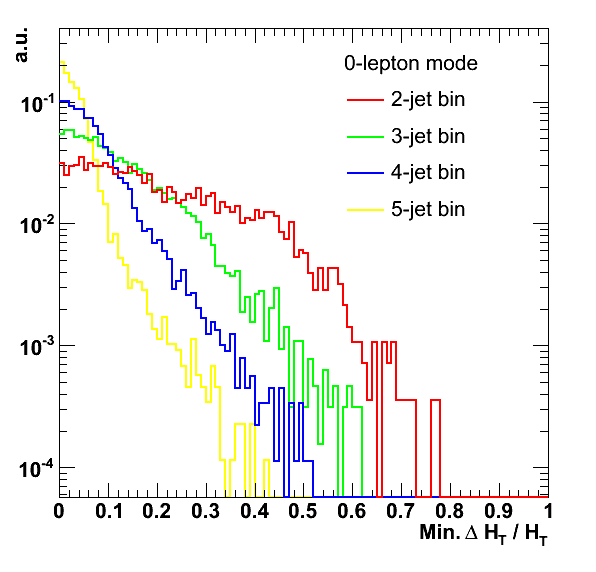
\includegraphics[scale=0.36]{./plots/dht_njet.png}}
\end{minipage}
\begin{minipage}[b]{0.5\linewidth}
\centering
{\label{fig:qcd_cor}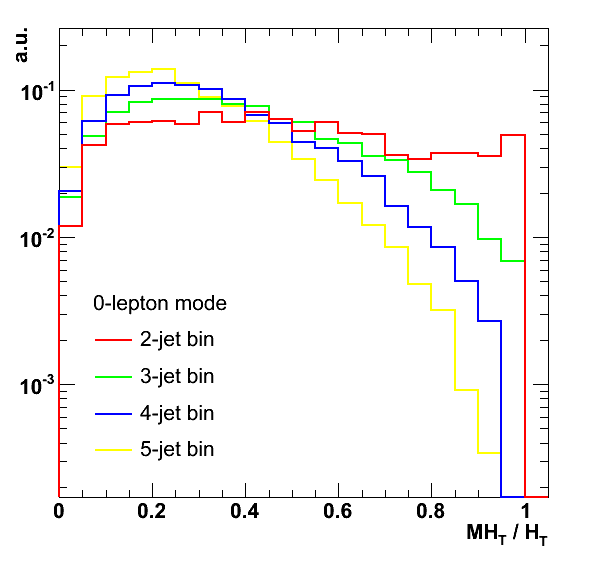
\includegraphics[scale=0.36]{./plots/mht_njet.png}}
\end{minipage}
\caption{\textit{The $\Delta H_{T}$ (left) and $MH_{T}$ (right) distribution at LM0, decomposed in N jet-multiplicity bins (N = 2, 3, 4, 5), for the all-hadronic channel.} }
\label{fig:obj-mult}
\end{figure}

\begin{figure}[h!]
\begin{minipage}[b]{0.5\linewidth}
\centering
{\label{fig:lm1_cor}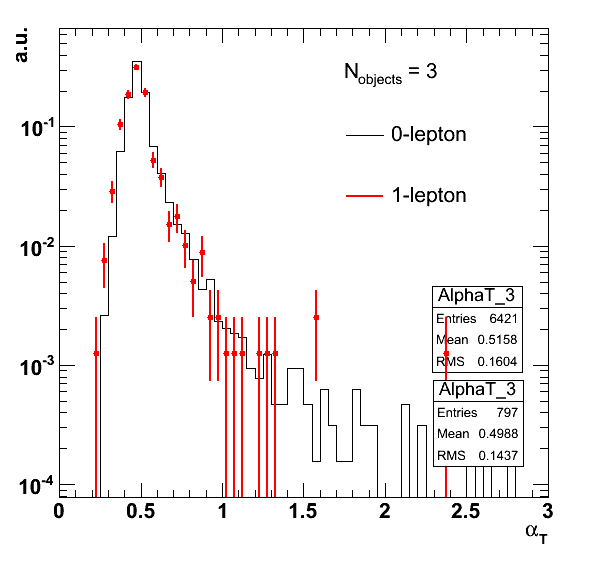
\includegraphics[scale=0.36]{./plots/aT_njet.png}}
\end{minipage}
\begin{minipage}[b]{0.5\linewidth}
\centering
{\label{fig:qcd_cor}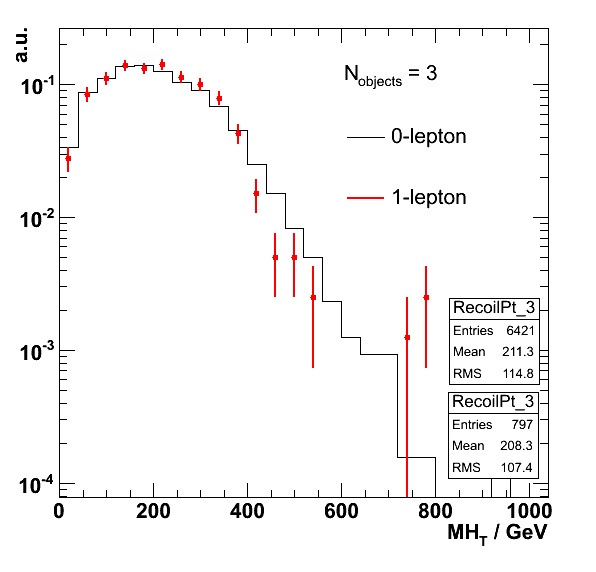
\includegraphics[scale=0.36]{./plots/recoil_njet.png}}
\end{minipage}
\caption{\textit{The $\alpha_{T}$ (left) and $MH_{T}$ (right) shapes at LM0, decomposed in object-multiplicity bins (N = 3, 4, 5 objects), for the all-hadronic and 1-lepton mode SUSY channels superimposed. }}
%The agreement in shape is obvious between the two channels, for the same object multiplicity - $N_{0-lepton}$ = n-jets and $N_{1-lepton}$=(n-1)-jet + 1-lepton.} }
\label{fig:kin}
\end{figure}


\begin{comment}
\begin{figure}[h!]
\begin{minipage}[b]{0.5\linewidth}
\centering
{\label{fig:lm1_cor}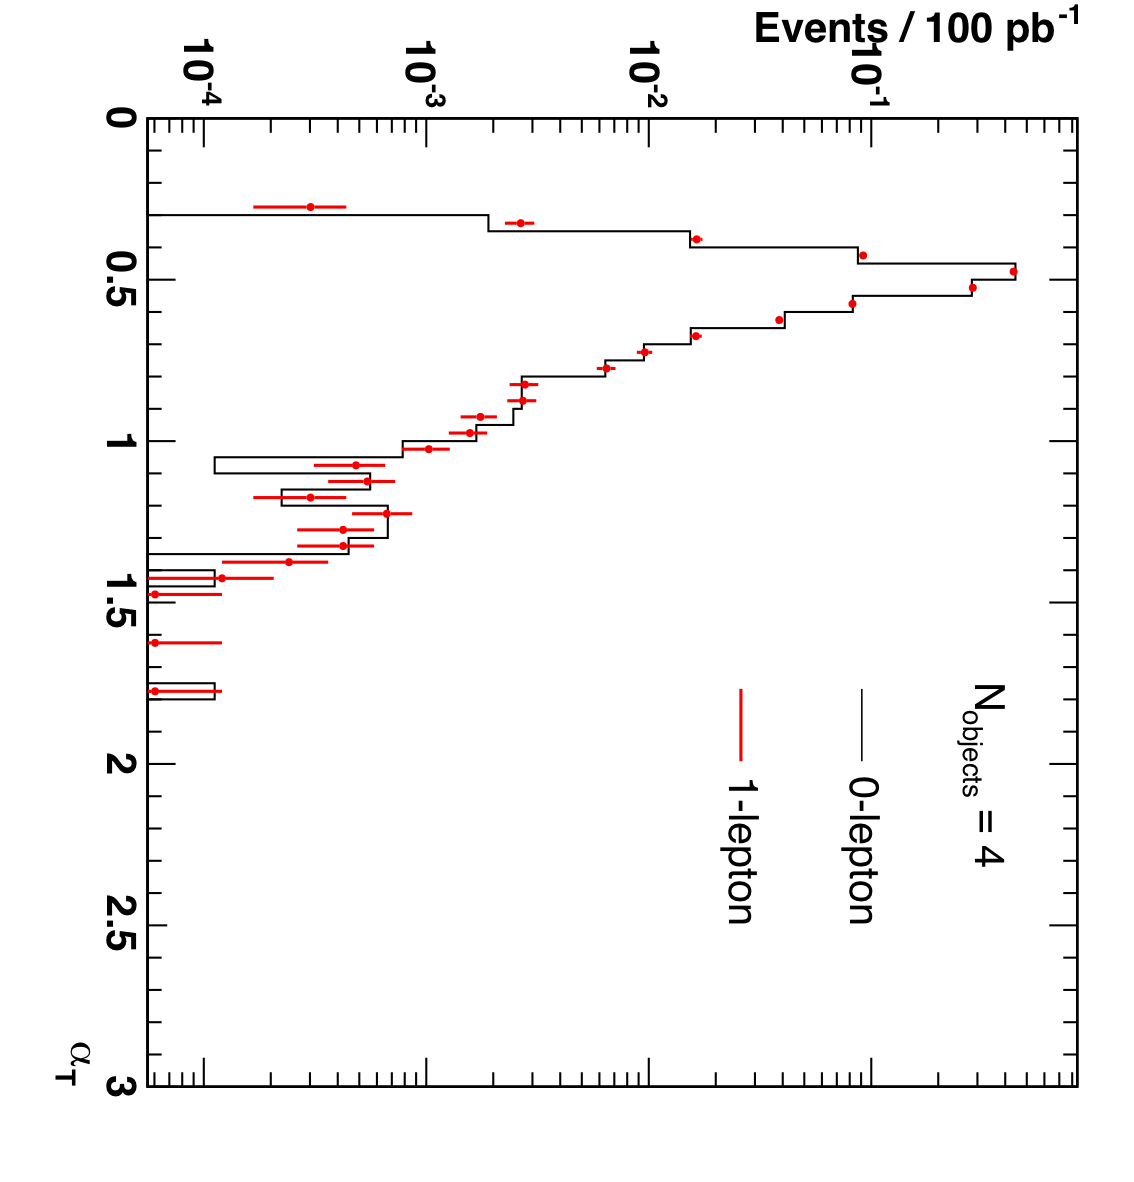
\includegraphics[scale=0.36, angle=90]{./plots/aT_4}}
\end{minipage}
\begin{minipage}[b]{0.5\linewidth}
\centering
{\label{fig:qcd_cor}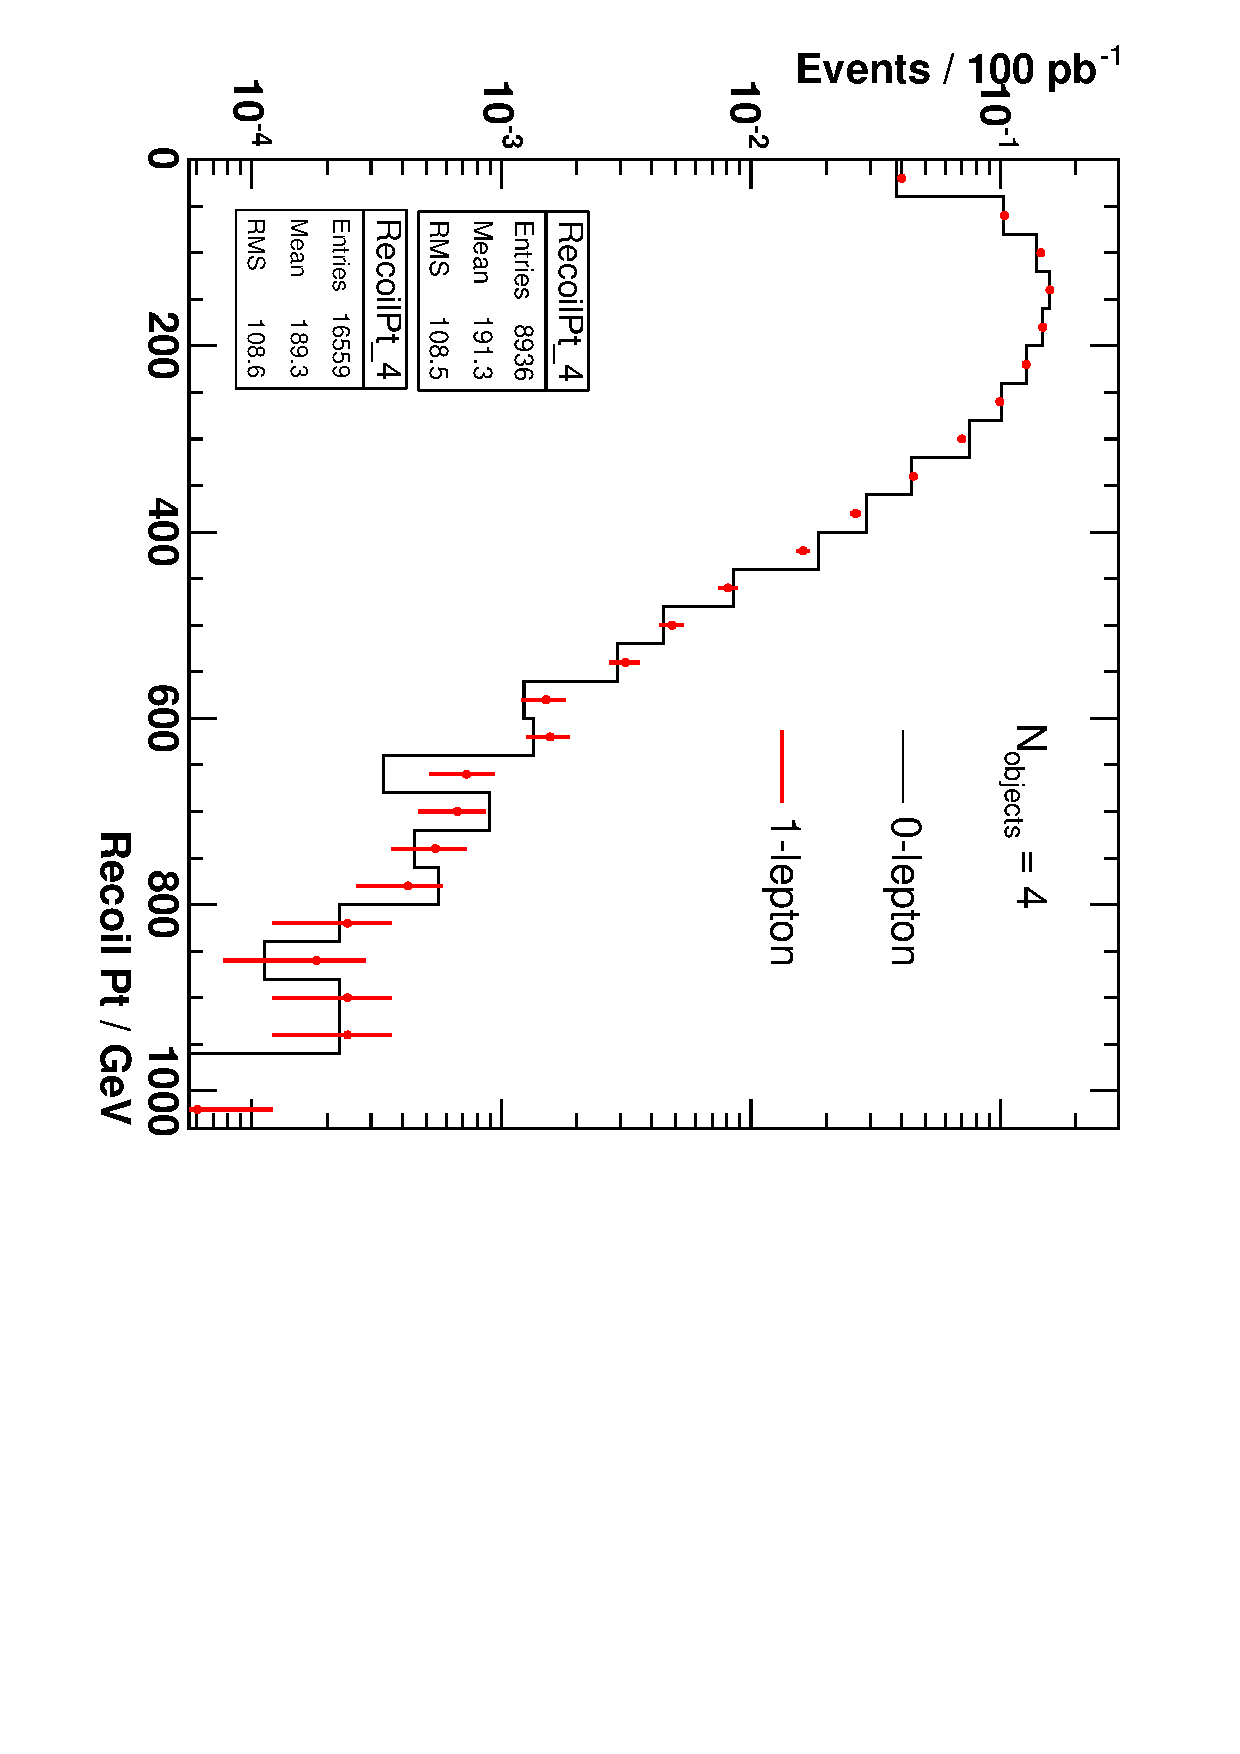
\includegraphics[scale=0.36, angle=90]{./plots/mht_4}}
\end{minipage}
%\caption{\textit{} }
\label{fig:cor}
\end{figure}
\begin{figure}[h!]
\begin{minipage}[b]{0.5\linewidth}
\centering
{\label{fig:lm1_cor}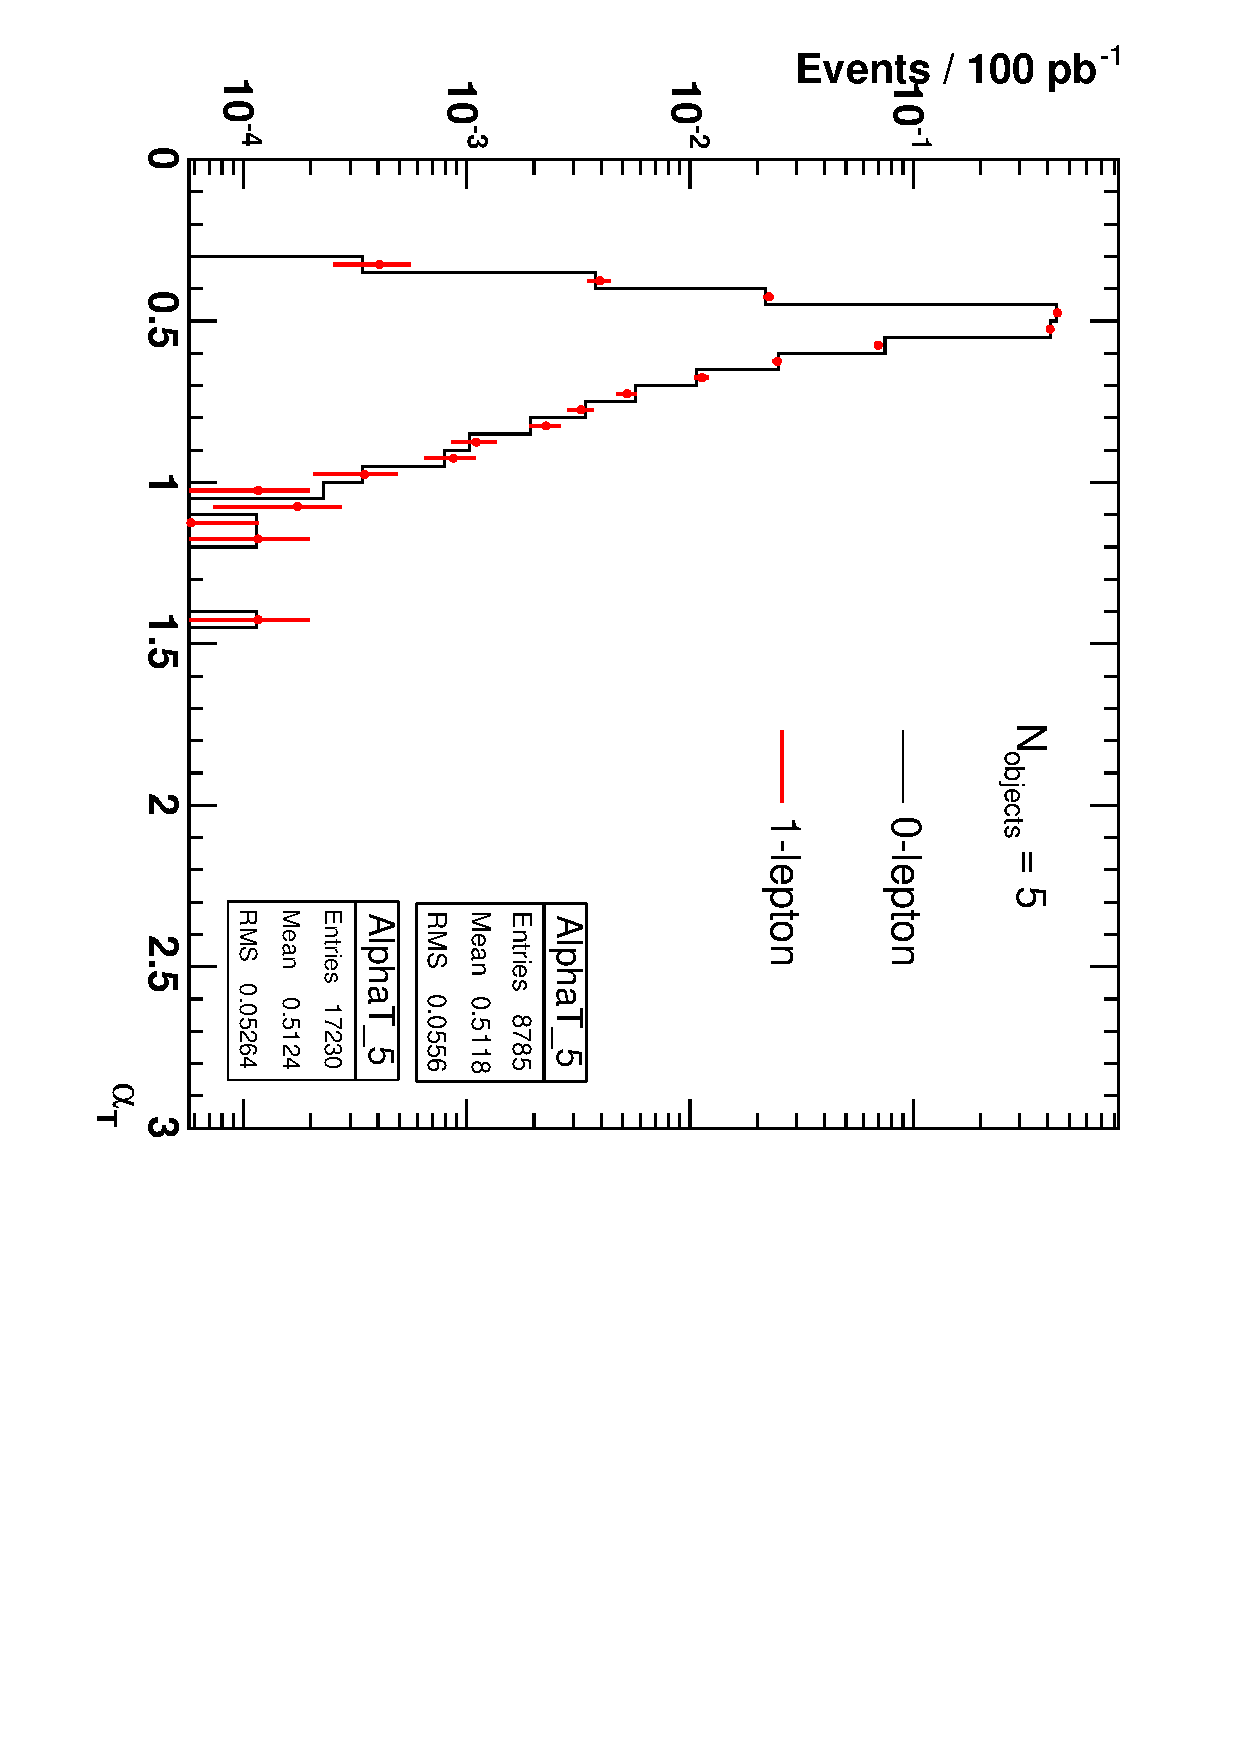
\includegraphics[scale=0.36, angle=90]{./plots/aT_5}}
\end{minipage}
\begin{minipage}[b]{0.5\linewidth}
\centering
{\label{fig:qcd_cor}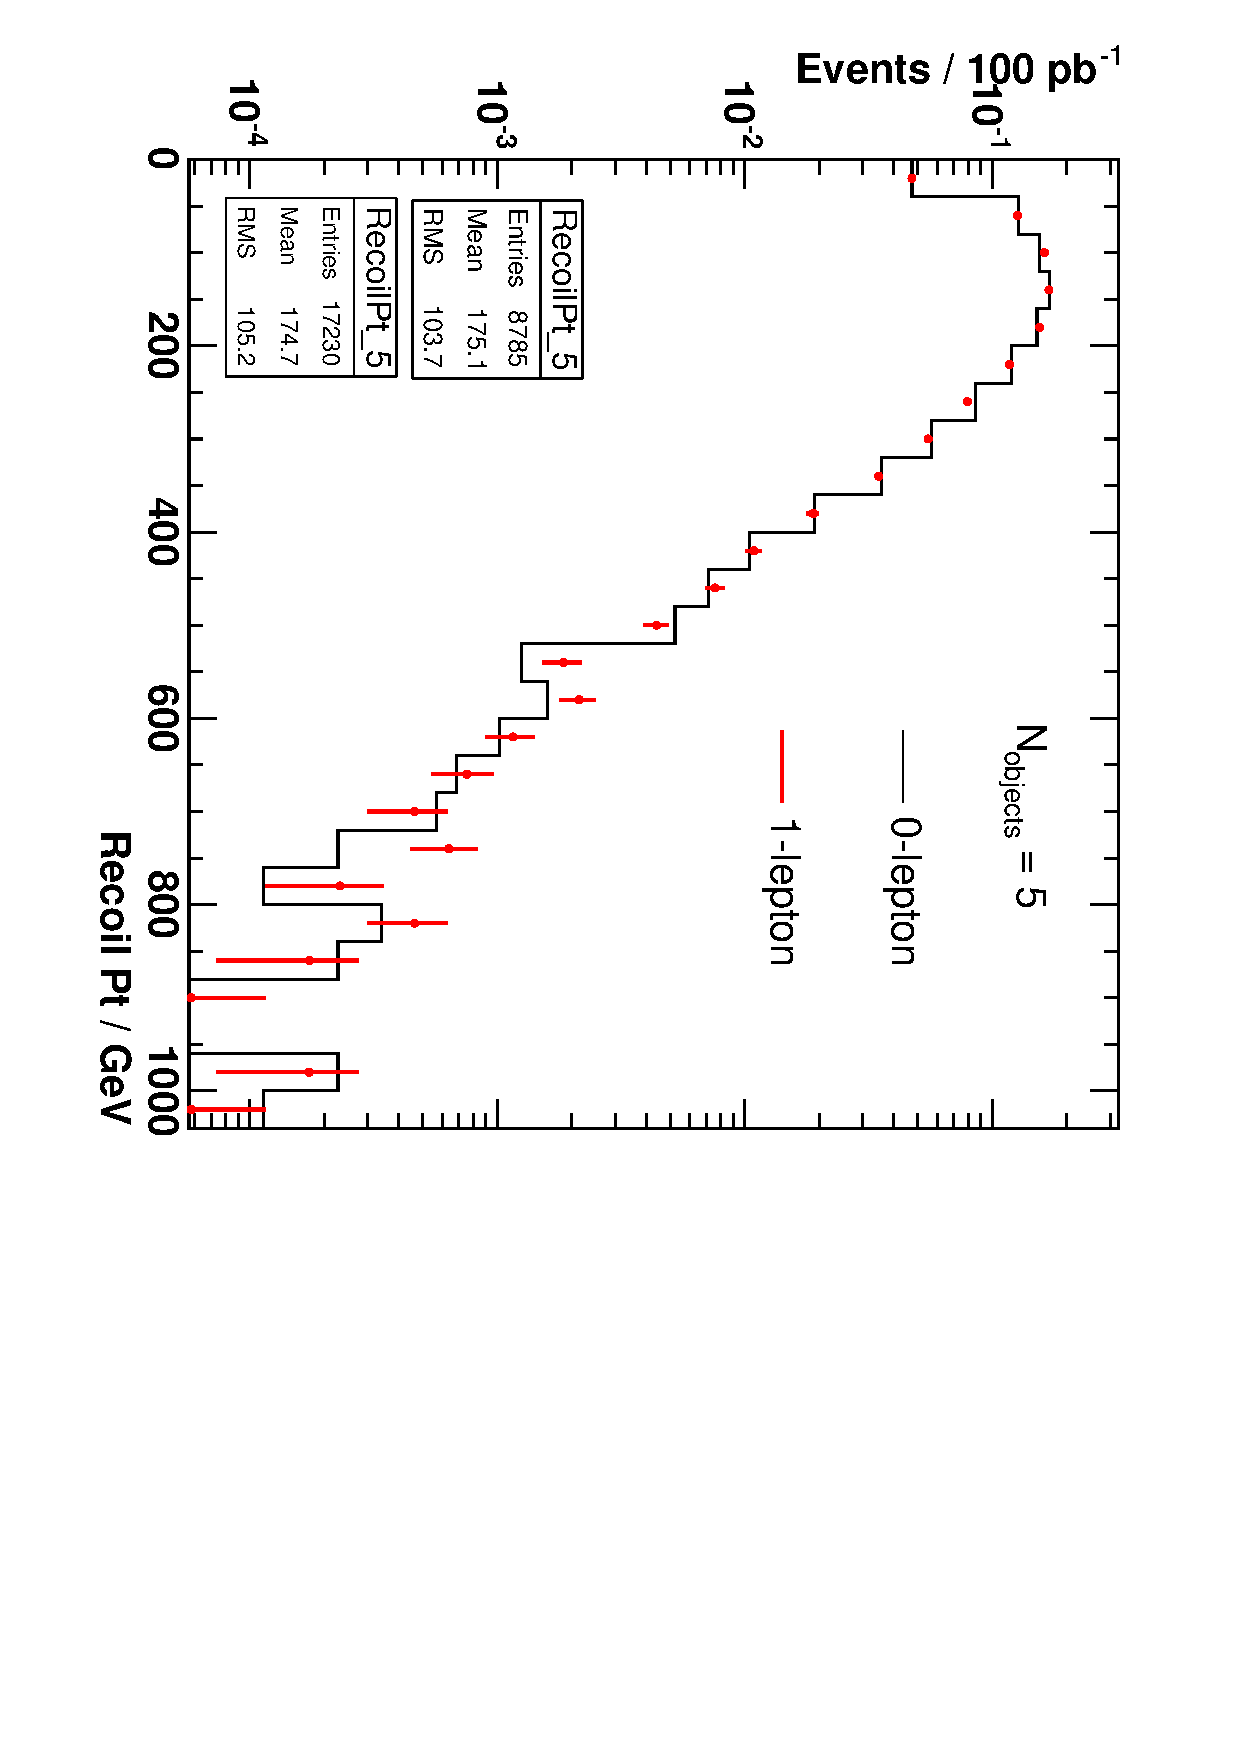
\includegraphics[scale=0.36, angle=90]{./plots/mht_5}}
\end{minipage}
\caption{\textit{\small {The $\alpha_{T}$ (left) and $MH_{T}$ (right) shapes at LM0, decomposed in object-multiplicity bins (N = 3, 4, 5 objects), for the all-hadronic and 1-lepton mode SUSY channels superimposed. The agreement in shape is obvious between the two channels, for the same object multiplicity - $N_{0-lepton}$ = n-jets and $N_{1-lepton}$=(n-1)-jet + 1-lepton.}} }
\label{fig:kin}
\end{figure}
\end{comment}

The ``leptonic'' version of the $\alpha_{T}$ variable is intended to control the QCD background which survives the one-lepton selection due to fake leptons or leptons from heavy-flavor decays. It has been shown to maintain the good performance in controling the QCD background as in the all-hadronic channel. This is illustrated in fig.~\ref{fig:cor}, which shows the correlation between the $\Delta H_{T}$ and $MH_{T}$ in the one-lepton channel, for the SUSY signal and the QCD N-jet background. One can notice that in the case of QCD (right plot), the correlation grows strong across the diagonal where the severe mismeasurements appear: large values of $\Delta H_{T}$ are grown along with large values of $MH_{T}$.

The functional form of the (leptonic) $\alpha_{T}$ is shown on the same figure for constant values equal to 0.55. It can be seen that the curve $\alpha_{T}>0.55$ is able to reject all of the QCD events, as expected.


\begin{figure}[h!]
\begin{minipage}[b]{0.5\linewidth}
\centering
{\label{fig:lm1_cor}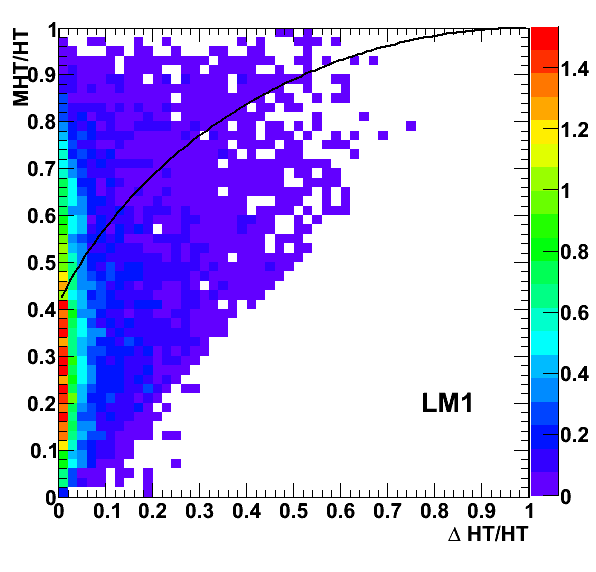
\includegraphics[scale=0.36]{./plots/lm1_cor.png}}
\end{minipage}
\hspace{3mm}
\begin{minipage}[b]{0.5\linewidth}
\centering
{\label{fig:qcd_cor}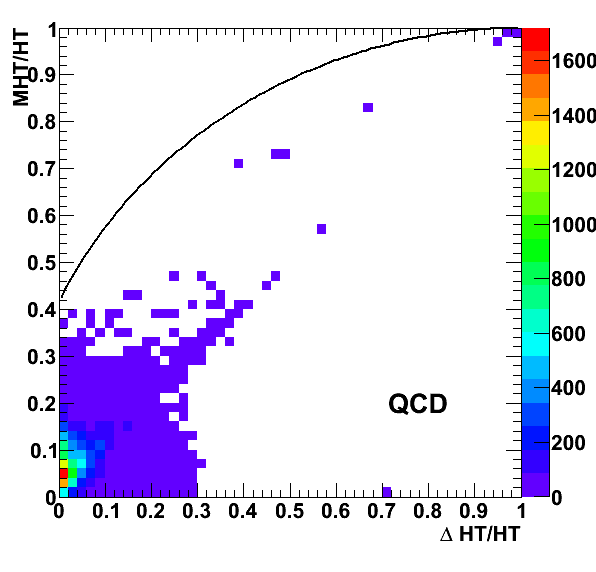
\includegraphics[scale=0.36]{./plots/qcd_cor.png}}
\end{minipage}
%\subfloat[LM1 events.]{\label{fig:lm1_cor}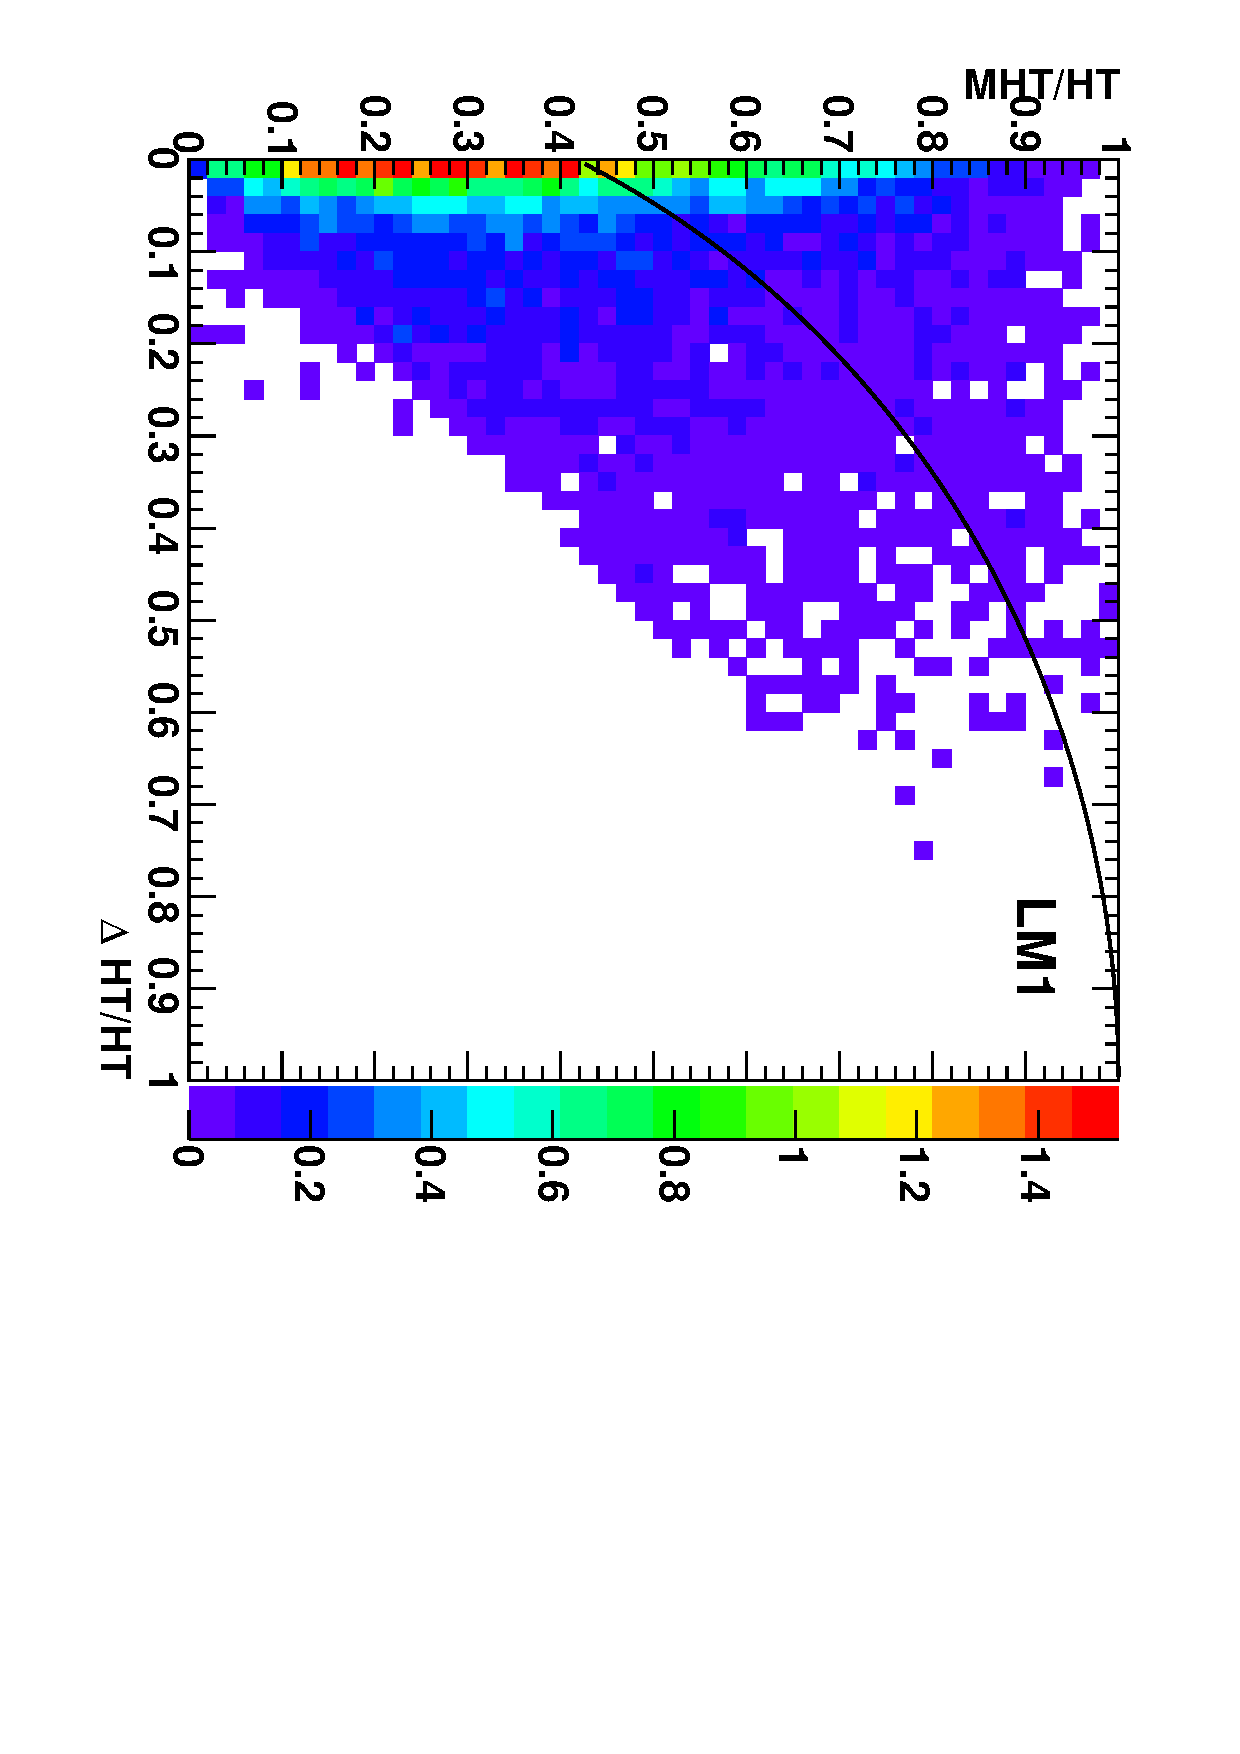
\includegraphics[scale=0.4, angle=90]{./plots/lm1_correlation_1lepton_afterHT}} 
%\subfloat[QCD plus $b\bar{b} + \textrm{jets}$ events.]{\label{fig:qcd_cor}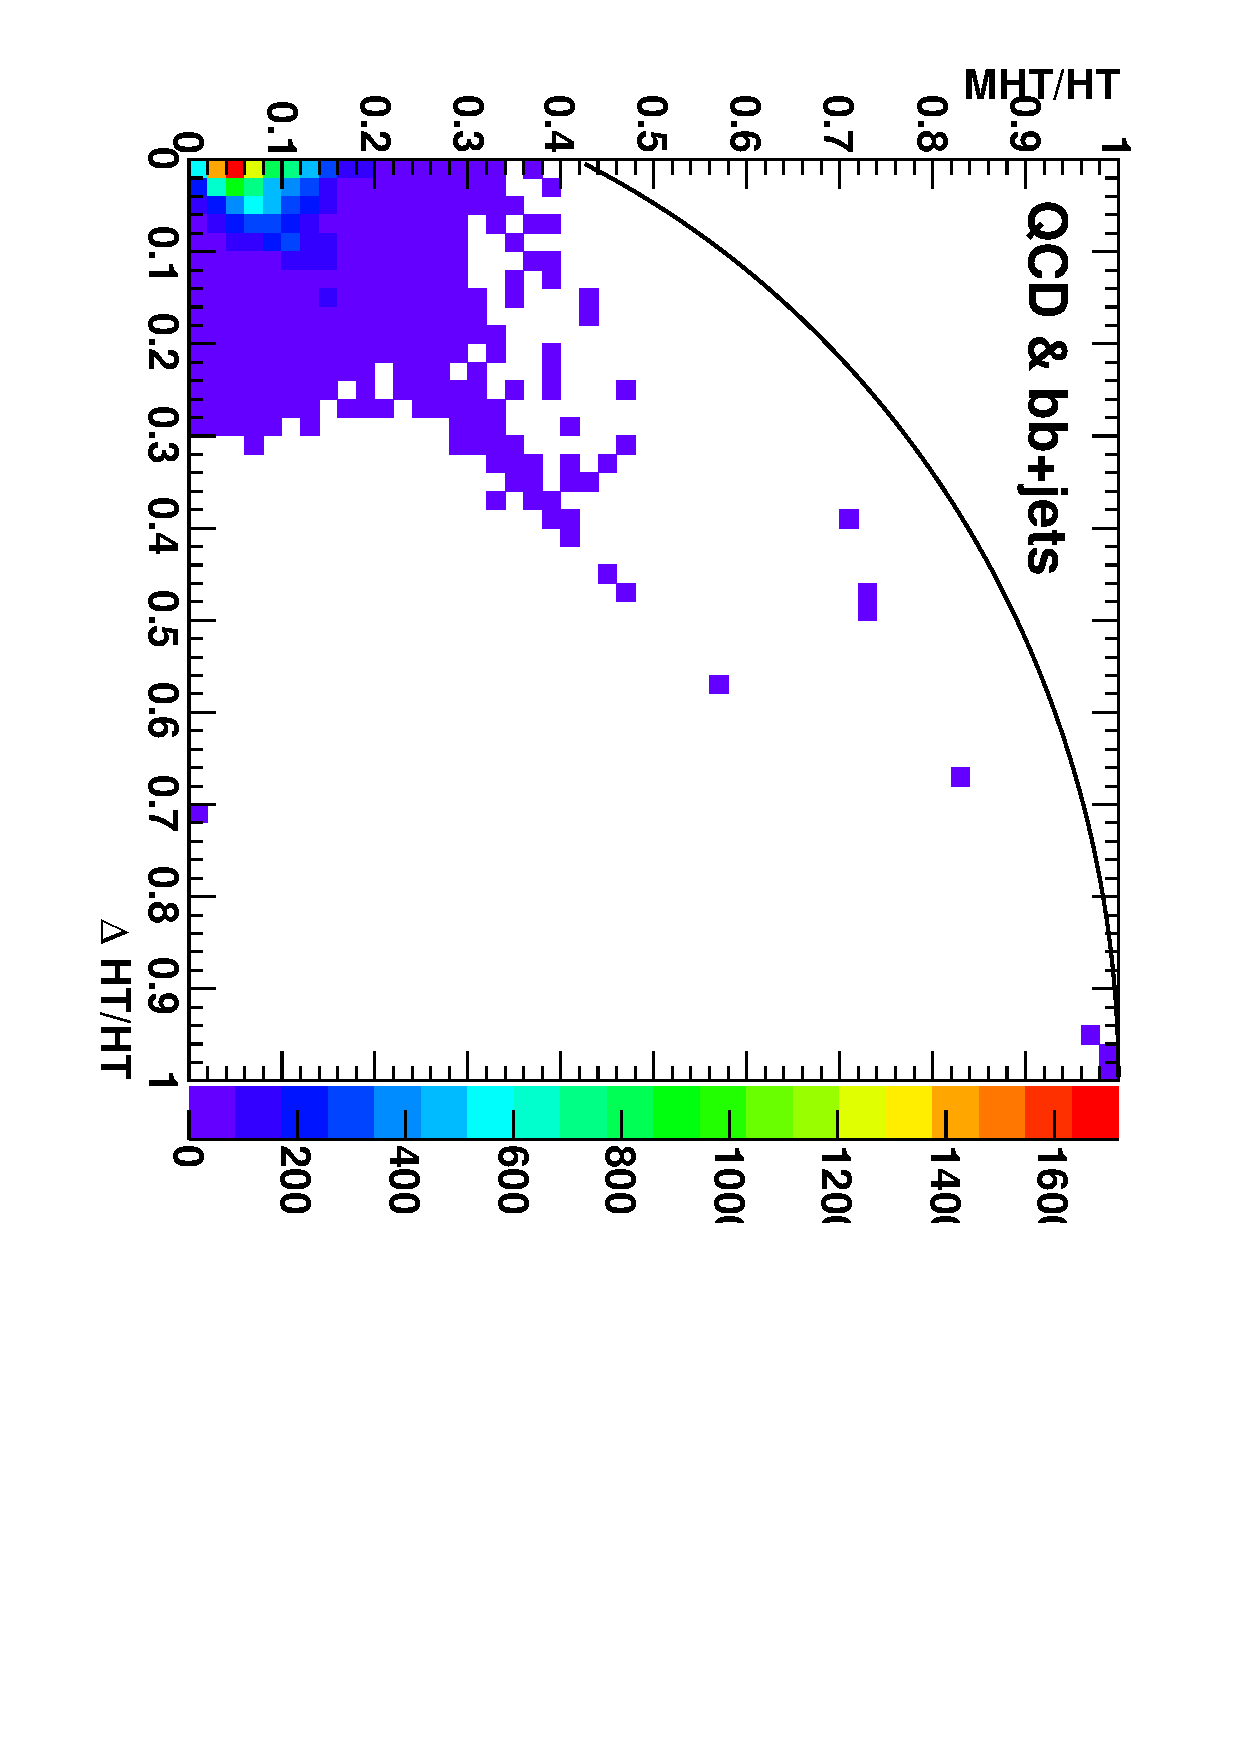
\includegraphics[scale=0.4, angle=90]{./plots/qcd_correlation_1lepton_afterHT}} 
\caption{\textit{The correlation of $\Delta H_{T}/H_{T}$ with $MH_{T}/H_{T}$ in SUSY LM1 events (a) and QCD events (b), in the 1-lepton mode channel. An $H_{T}$ cut of 350 GeV has been applied. The black line indicates constant values of $\alpha_{T}=0.55$.} }
\vspace{5mm}
\label{fig:cor}
\end{figure}